\documentclass[english]{scrartcl}
\usepackage{babel}
\usepackage[margin=1.1in]{geometry}
\usepackage[utf8]{inputenc}
\usepackage{bm}
\usepackage{hyperref}
\usepackage{amssymb}
\usepackage{amsmath}
\usepackage{parskip}
\usepackage{enumitem} % para poder empezar con 0 el enumerate
\usepackage{soul}
\usepackage{graphicx}

\hypersetup{
	pdftitle={APA - Practical Work Report},
	colorlinks=true, % Use colours instead of boxes.
	urlcolor=blue
}

\newcommand\ms[1]{\texttt{#1}}
\newcommand\R[1]{\texttt{#1}}
\soulregister{\ms}{1}
\soulregister{\R}{1}

\begin{document}
\thispagestyle{empty}
\begin{center}

\vspace*{\fill}

{\bf\LARGE APA - Practical Work Report}
\par \vspace{6mm}
{\LARGE FIB - 2012-2013 Q1}

\par 
\par\vspace{3mm}

{\bf 
    Alejandro Fernández Suárez\\
    Marc Sunet Pérez
}

\par\vspace{5mm}
{\bf\LARGE Census Income Classification}
\vspace{3mm}

\vspace*{\fill}

\end{center}

\newpage

\vspace*\fill

\thispagestyle{empty}
\tableofcontents

\vspace*\fill

\newpage
\setcounter{page}{1}
\section{Description of the problem and available data}

The problem consists in creating a model that predicts whether a given individual makes \$50K or more a year. Training and testing data has been obtained from \url{http://archive.ics.uci.edu/ml/datasets/Census+Income}.

Each individual in the data set specifies a set indicators such as age, work class and education, from which the yearly income has to be predicted. Our goal is to make that prediction, to tell which variables the target variable is truly dependent on and to analyse the results. In the process, we test different machine learning algorithms and compare the quality of their outputs.

\section{Data pre-processing}

Our dataset comes from a discrete census information table, meaning that no values come from continuous/noisy sources such as image, sound or video and that therefore no tinkering has to be performed on the input values.

The only transformation we apply to the input is the conversion of categorial fields such as race and sex to numerical values and the conversion of the target variable to a factor. These two steps are needed by all of the classification models that we build, which is why we perform them as part of the pre-processing.

\section{Models}

The problem at hand is a binary classification one and we have therefore chosen appropriate models for this task, namely LDA/QDA, MLP neural networks, logistic regression and SVMs. In the following sections we describe the procedure used to build each of the models.

    \subsection{LDA/QDA}
    
    \subsubsection{Regularization and dataset partitioning for LDA and QDA}
    As we'll see in section \ref{sec:methods:ldaqda}, we use Leave-One-Out Cross Validation to get the best linear and quadratic classification models we 
    can. The data set is partitioned in learning and testing subsets to check the accuracy of the methods without using LOOCV.
    
    \subsubsection{Linear and Quadratic Classification Models}
    \label{sec:methods:ldaqda}
    Both Linear and Quadratic Discriminant Analysis models are validated using
    half of the samples of the original dataset. The half of the data used for training (model creation) is composed by
    randomly selected samples. The second half is composed by the samples not in the training set and it's called the 
    testing set. Both Linear and Quadratic models are analyzed and validated predicting the learning dataset and the test
    dataset. Regularized models are finally obtained using Leave-One-Out Cross Validation, giving place to more robust
    and reliable classifiers.
    
    \subsection{MLP Neural Network}
    \label{sec:methods:nnet}
    We have built two neural network models. The first one uses all the input data, while the second uses only the most
    relevant features of the input, as analyzed previously.
    
    \subsubsection{MLP Neural Network hidden units analysis}
    For the case of the MLP neural network, the non-linear model obtained is validated by just predicting the training set. However, for both models obtained
    (see section \ref{sec:methods:nnet}), we analyze which is the best number of hidden units from 1 up to 10. The results obtained will be shown in detail in
    section \ref{sec:results:nnet}.
    
    \subsection{Logistic Regression}
    An initial model is built from the entire data set. We then find out which variables the target is dependent on and we build a second model using only these variables. This second model is compared against the first one to verify that the variables that have are discarded are indeed irrelevant to predict the target variable.
    
    Using the selected variables only, we then apply k-fold cross-validation for different values of k to obtain a set of different models, as well as leave-one-out cross-validation to obtain a last one.
    
    \subsection{SVM}
    Different SVM models are built from the data set. First, we build linear, polynomial and radial models from the entire data set. Then, we apply 3-fold cross-validation and obtain another set of models for each of the test/trainining partitions. The models are then compared to see which one performs the best.

\section{Results}

    \subsection{Linear and Quadratic Classification Models}
    Given the nature of the problem, linear and quadratic classification models give good enough results because the influence
    of each input parameter is not bound to the values of the rest of parameters. Since there are many different input parameters,
    linear and quadratic models work good at balancing the weight of each input on the final results. Aaccuracy rates obtained for each model and testing set are shown in table \ref{table:ldaqda-results}.
    
    \begin{table}[h]
    \centering
    \begin{tabular}{l c}
    \textbf{Model} & \textbf{Accuracy} \\
    LDA - Resubstitution of the learning data set & ~76\% \\
    LDA - True accuracy using testing set & ~58\% \\
    LDA - Regularized (LOOCV) model & ~77\% \\
    QDA - Resubstitution of the learning data set & ~81\% \\
    QDA - True accuracy using testing set & ~68\% \\
    QDA - Regularized (LOOCV) model & ~82\% \\
    \end{tabular}
    \caption{Results for LDA/QDA models.}
    \label{table:ldaqda-results}
    \end{table}
    
    As we can see, the quadratic methods a fairly better results compared to the linear ones for our problem.
    
    \subsection{MLP Neural Network}\label{sec:results:nnet}
    The non-linear models we get using neural networks don't show special good features due again to the nature of the problem itself.
    As we'll go on, we'll see that our problem can be modelled in a good enough way using linear methods. Thus, non-linear models provide
    good solutions too, but don't show any special qualities with respect to the linear approaches. These are the results obtained for
    our neural networks:
    \begin{itemize}
    \item Using all inputs: The best accuracy obtained is ~77\% with 7 hidden units
    \item Using only the most relevant inputs: The best accuracy obtained is ~79\% with 9 hidden units
    \end{itemize}
    
    \subsection{Logistic Regression}
    Results for the logistic regression models are summarised in table \ref{table:logit-results}.
    
    \begin{table}[h]
    \centering
    \begin{tabular}{l c}
    \textbf{Model} & \textbf{Error rate} \\
    Initial & 0.2430621 \\
    Initial (bin) & 0.1749079 \\
    Pruned & 0.2431116 \\
    Pruned (bin) & 0.1753993 \\
    2-fold & 0.2450596 \\
    3-fold & 0.2432385 \\
    4-fold & 0.2439326 \\
    5-fold & 0.2438422 \\
    6-fold & 0.2447852 \\
    \end{tabular}
    \caption{Results for logistic regression models.}
    \label{table:logit-results}
    \end{table}
    
        
    \subsection{SVM}
    The results obtained from the SVM models are the ones shown in table \ref{table:svm-results}.
    
    \begin{table}[h]
    \centering
    \begin{tabular}{l c}
    \textbf{Model} & \textbf{Error rate} \\
    Linear & 0.1848894 \\
	Polynomial & 0.1511978 \\
	Radial & 0.1437654 \\
	Linear-CV1 & 0.1870278 \\
	Polynomial-CV1 & 0.1566243 \\
	Radial-CV1 & 0.1512806 \\
	Linear-CV2 & 0.1851852 \\
	Polynomial-CV2 & 0.1579141 \\
	Radial-CV2 & 0.1517413 \\
	Linear-CV3 & 0.1836359 \\
	Polynomial-CV3 & 0.1612457 \\
	Radial-CV3 & 0.1535059 \\
    \end{tabular}
    \caption{Results obtained from the different SVM models.}
    \label{table:svm-results}
    \end{table}
    
    The models labeled \ms{Linear}, \ms{Polynomial} and \ms{Radial} correspond to the models obtained using leave-one-out cross-validation. The ones labeled \ms{Linear-CVi}, \ms{Polynomial-CVi} and \ms{Radial-CVi} for $i \in \{1,2,3\}$ are the ones obtained using 3-fold cross-validation.
    
    As we can see, even though it seems the input is not linearly separable, it does seem to be close enough, as the differences in error rates between the linear and polynomial models are very tight. Furthermore, it is worth noting that the radial models do not present a significant improvement over the polynomial ones, so we conclude that the input data can be separated both polynomically and linearly, although not without making a few extra errors in the latter case.

\section{Method Comparison}

As we can see in figure \ref{fig:results}, no model outbeats the others by far in terms of
accuracy on the prediction. However, there are a few aspects to take into account when
it comes to decide which one fits better for our problem:

\begin{figure}[h!]
 
  \centering
    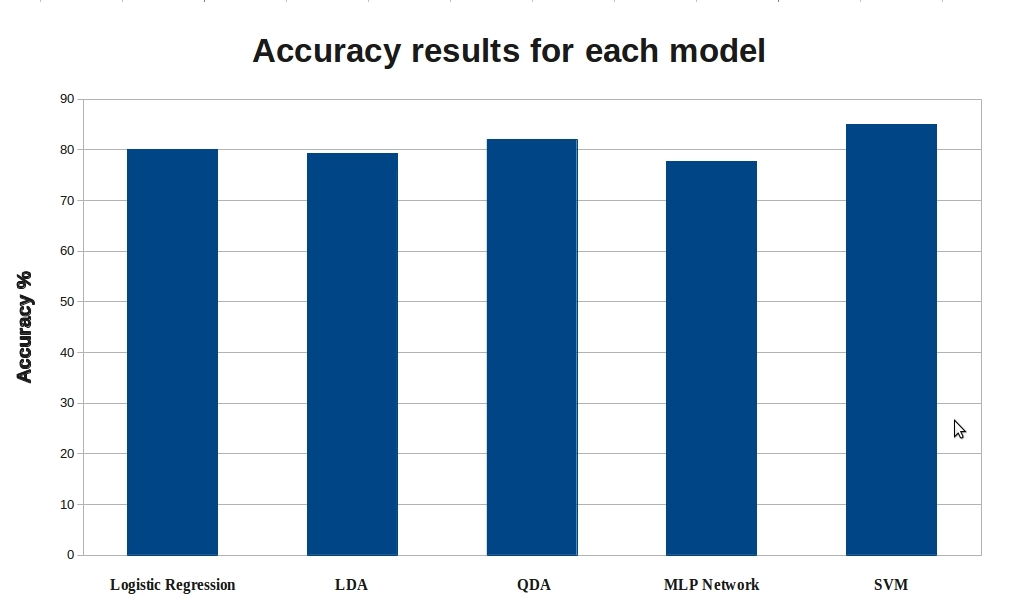
\includegraphics[width=1\textwidth]{results}
   \caption{Model accuracy comparison}
   \label{fig:results}
\end{figure}

\begin{itemize}
\item The logistic regression is hard and expensive to validate and test in this 
problem due to the relatively large amount of input parameters we get, even after
filtering. This makes the models obtained by logistic regression the first ones 
in being discarded.

\item The non-linear approaches don't show any special improvement with respect
to the linear models, so we can accept a good linear model for simplicity.

\item The leave-one-out cross validation used in LDA and QDA gives more stable
and reliable models with respect to the ones that have been tested by just folding.

\item In terms of accuracy, the best model obtained is an SVM, with an accuracy
of 84.5 \% and it has been assessed by cross-validation.

\item Although we have determined the optimum number of hidden units for the 
MLP neural networks, they show no improvement on prediction accuracy, so we
are very likely going to choose another approach as a final model.
\end{itemize}

\section{Final Model and Generalisation Error}

The \texttt{Radial-CV1} model is the best model we have obtained from the data set, which corresponds to an SVM with a radial kernel trained with 3-fold cross validation. 

It is worth noting, however, that error rate of the \texttt{Radial-CV1} model is not execessively better than that of the other SVMs, or even the QDA model trained with leave-one-out cross validation. This, and the fact that the polynomial methods are quite close to the linear ones, seems to suggest that the data forms a very big circle, so big that the data is locally linear.

From the training of the logistic regression models, we have learned that an individual's country of residence is not a relevant factor towards determining the individual's yearly income. To confirm this, we analyse the data set and figure out which of the given countries have individuals that earn more than \$50K a year. As it turns out, only 2 of the 42 input countries fail to satisfy this condition, suggesting that the country is indeed irrelevant, or at least neglectable.

The final model is then a radial SVM model trained with 3-fold cross validation after discarding the country attribute of the input data. The prediction error rate given by this model is of 15\%, meaning that the model correctly predicts the target variable 85\% of the times.

\section{Conclusions}

A given individual's country of residence is not a relevant factor towards determining their yearly income. The given data is technically not linearly separable, but if we allow some error we can get decent linear estimates. The polynomial models do only slightly better, and the radial present a neglectable gain ($<1\%$) with respect to the polynomial ones, suggesting that the data set is locally linear.

\end{document}
